\chapter{Summary and future directions: preliminary and proposed studies of circadian control}

The prior two chapters have presented preliminary theoretical studies of circadian control.
The first result, a comparison of optimal with model predictive control, presents an important benchmark for the performance of any applied control scheme, and uses this to identify how MPC design parameters affect control optimality.
The second result proposes a method for controlling populations of oscillators without adversely affecting population synchrony.
While these propose a path toward translational closed-loop circadian control, there are remaining challenges before either may be implemented.

Herein, I briefly discuss future research directions toward the control of circadian rhythms.
The first of these is the development of a real-time sensor of circadian phase, an essential development for circadian control in ambulatory conditions.
The second proposed direction involves improving control abilities by relaxing the assumption that the oscillator stays near its limit cycle.
By relaxing this assumption, we may shift the oscillator closer to its fixed point, where phases are more condensed in state space, and therefore may be shifted between more easily.

\section{Closing the loop: development of a circadian phase sensor}

Although we have made significant progress in developing control algorithms for circadian oscillation, there remains significant barriers to achieving closed-loop control in clinical settings.
Most prominently, there is little current capability for real-time sensing of circadian phase, and even less ability when invasive or expensive methods are excluded.
Open loop control does not require sensing of phase, and therefore it has been used exclusively to-date in publicly available phase resetting protocols \cite{Walch2016}.
The ability of feedback control to overcome imprecise modeling and poor model assumptions arises directly from the incorporation of feedback, and so sensing phase is an essential component of more advanced control systems.
In clinical settings, circadian phase is generally assessed by salivary or blood melatonin levels, core body temperature (as recorded from a rectal thermometer), or, rarely, cortisol levels \cite{Klerman2002, Chang2012a, StHilaire2012}.
While these techniques allow precise phase calculations in clinic, they are insufficient for ambulatory settings and prohibitively invasive for widespread adoption.

There has been a recent push to use machine learning techniques to sense circadian phase from ambulatory data; for example, recent studies have combined skin temperature sensors and actigraphy recordings to estimate phase \cite{Kolodyazhniy2011, Kolodyazhniy2012}.
Machine learning methods have shown promise and improved performance in comparison simple multiple regression models, with the majority of phase estimates within $\pm0.3$ radians (approximately 1 h).
In these cases, the actigraphy recordings provided little utility in comparison to the skin temperature sensors \cite{Kolodyazhniy2012}.
However, actigraphy data is the most readily available to the average individual through motion sensing in smartphones or smartwatches.
An improved approach might include sampling the individual's ambient light environment in addition to activity.
Data of this sort have already been collected by the Klerman lab at Harvard Medical School/Brigham and Women's Hospital from a cohort of approximately 150 college undergraduates.
A logical next step would be using machine learning to estimate continuous phase from this dataset, and compare with clinical phase measurements.

A potentially helpful approach in linking the sensor to the control algorithm would be the use of a confidence index, a scalar metric describing the historical accuracy of phase prediction given the input data \cite{Laguna2017}.
In this case, the confidence index could indicate a high degree of certainty in the estimated phase, or if the confidence in phase estimation is low, a high degree of certainty regarding the predicted response (i.e.\ if all likely phases result in the same phase shift).
This metric would then be used to tune the aggressiveness of the controller or the sampling rate.
A simple confidence index would, for example, stop control action when in the vicinity of ipPRC zero crosses, to prevent accidentally shifting the phase in the non-optimal direction.
Approaches such as those in Chapter 6 could be used to similarly find bounds on the error incurred due to imprecision in the phase estimation, and these calculations would dictate how the confidence index would be incorporated into the controller.

When combined with the MPC approaches from the prior two chapters, the development of a phase sensor will enable the first closed-loop control of circadian phase.
Though there are no current plans to perform closed-loop human circadian control experiments, I anticipate that closed-loop circadian control will be feasible in a clinical setting within the next five years.
Aside from circadian control, the ability to sense circadian phase has potential benefits in other aspects of precision medicine.
For example, the majority of common pharmaceuticals target clock products, and circadian phase affects the pharmacokinetic and pharmacodynamic properties of nearly any therapeutic, since RNA abundance of about 40\% of protein-coding genes are thought to cycle with a circadian rhythm \cite{Zhang2014a}.
Thus, the ability to accurately and noninvasively assess circadian phase is critical for the development of next-generation dynamic drug delivery strategies.

\section{Critical-resetting MPC: leveraging the limit-cycle fixed point}

\subsection*{Introduction}
When developing controls methods for manipulating circadian phase, we made the decision to reduce the limit-cycle oscillator model to a phase-only formulation.
In doing so, we reduced the dimensionality of state space from $n$ dimensions to a single dimension.
This allowed simple use of the phase response curve to identify when the oscillator would be phase-delayed or phase-advanced by the stimulus.
We applied control based off the ipPRC we calculated, and referred to such a PRC as ``type 1.''
For large perturbations, or in some cases repeated perturbations \cite{Kronauer1999}, a ``type 0'' PRC has also been observed \cite{Czeisler1989}.
A type 0 PRC (called so because the mean slope of the phase transition curve, or PTC, is 0) contains a discontinuity resulting from the large magnitude phase shifts it describes.
This discontinuity mathematically arises from the oscillator being shifted far from the limit cycle in state space, and as a result, only having access to a subset of all possible final phases.

Type 0 resetting that results from the oscillator being pushed close to the critical point (from here, called ``critical resetting'') has an additional feature: a sustained reduction in the amplitude of circadian processes such as melatonin or core body temperature rhythms, which reverts to the pre-stimulus amplitude very slowly \cite{Jewett1994, Kronauer1999}.
The critical point is without phase, and correspondingly, individuals that have been shifted sufficiently near this point may be easily phase shifted into any desirable final phase.
Thus, it is feasible to design a ``critical MPC'' protocol for achieving large phase shifts by first forcing the individual to the critical point, then aligning them with the desired final phase.
However, this violates the phase-only assumption of the prior chapters.

A further to-date unexplained curiosity from these early studies of human circadian phase and amplitude resetting is that only a fraction ($\approx25$\%) of individuals respond to an identical series of stimuli with a critical resetting.
The preliminary work in this section sought to first explain this result, and in doing so, determine if critical resetting may be more widely achieved and used in circadian control. 


\subsection*{Modeling light input to the human circadian oscillator}

The most widely-used model of the circadian clock was developed by Kronauer and his collaborators nearly two decades ago \cite{Jewett1998,Kronauer1999}.
This model incorporates two processes.


Process P is a limit cycle oscillator, modified from the van der Pol oscillator, intended to capture endogenous circadian oscillation.
The two states of process P are given by:
\begin{equation}
    \frac{dX}{dt} = \left(\frac{\pi}{12}\right)\left(X_c + \mu \bigg(\frac{1}{3}X + \frac{4}{3}X^3 - \frac{256}{105}X^7\bigg) +B(t)\right) 
\end{equation}
\begin{equation}
    \frac{dX_c}{dt} =\left(\frac{\pi}{12}\right)\left(qB(t)\bigg(\frac{24}{0.99729\tau}\bigg)^2 X_c X + kB(t)X\right)
\end{equation}
where $X$ represents core body temperature, and $X_c$ is a non-biological co-state that drives oscillation.
Parameter $\tau$, here, is the period of oscillation, which may be selected \textit{a priori} and is typically set to $24.2$ h, to correspond with the human circadian period \cite{Czeisler1999}.
The kinetic parameters $\mu$, $q$, and $k$ do not have biological significance beyond parameterizing the shape of the limit cycle and are given in \cite{Kronauer1999}.
Term $B(t)$ is the photic drive, which is determined by process L.

Process L describes the dynamic effect of light input into the oscillator.
Experiments where light pulses were applied for varying durations and with varying spacing have shown that light response is pseudosaturating.
That is, the initial response to the pulse evokes a large-magnitude shift.
Continuing the light stimulus for a longer duration yields diminishing returns, until a constant, low level of drive is reached.
This response can be captured by modeling the dynamics of a population of light receptors, where $n(t)$ are the fraction of the population that is inactive, and $1-n(t)$ are active.
The conversion between active and inactive states is given by
\begin{equation}
    \frac{dn}{dt} = 60(\alpha(t)(1-n) - \beta n)
\end{equation}
where $\alpha$ and $\beta$ are the kinetic rates of inactivation and activation, respectively.
Thus, after a constant, sustained pulse, the fraction of the population that is active is given by $n_\infty = \alpha/(\alpha+\beta)$, yielding the pseudosaturation.
The kinetic term $\alpha$ is a function of light intensity, given by
\begin{equation}
    \alpha(t) = \alpha_0 \left(\frac{I}{I_0}\right)^p.
\end{equation}
The light drive from the receptors, $\hat B(t)$, is then a function of light intensity and the fraction of active states:
\begin{equation}
    \hat B(t) = G\alpha(t)(1-n(t)).
\end{equation}
Because the clock is more sensitive to light at certain phases, $\hat B$ is rescaled by the photic sensitivity state of the oscillator, to yield the effective light drive term $B(t)$:
\begin{equation}
    B(t) = (1-0.4X)(1-0.4X_c)\hat B(t),
\end{equation}
which is incorporated in process P.
The techniques used for fitting this model are explained in detail in \cite{Kronauer1999}.

Importantly, this model was fit to exhibit critical resetting in response to three five-hour pulses centered at the core body temperature ($X$) minimum (corresponding to approximately 5AM local time).

\subsection*{Inter-individual period variability explains critical resetting prevalence}

\begin{figure}[p]
    \begin{center}
        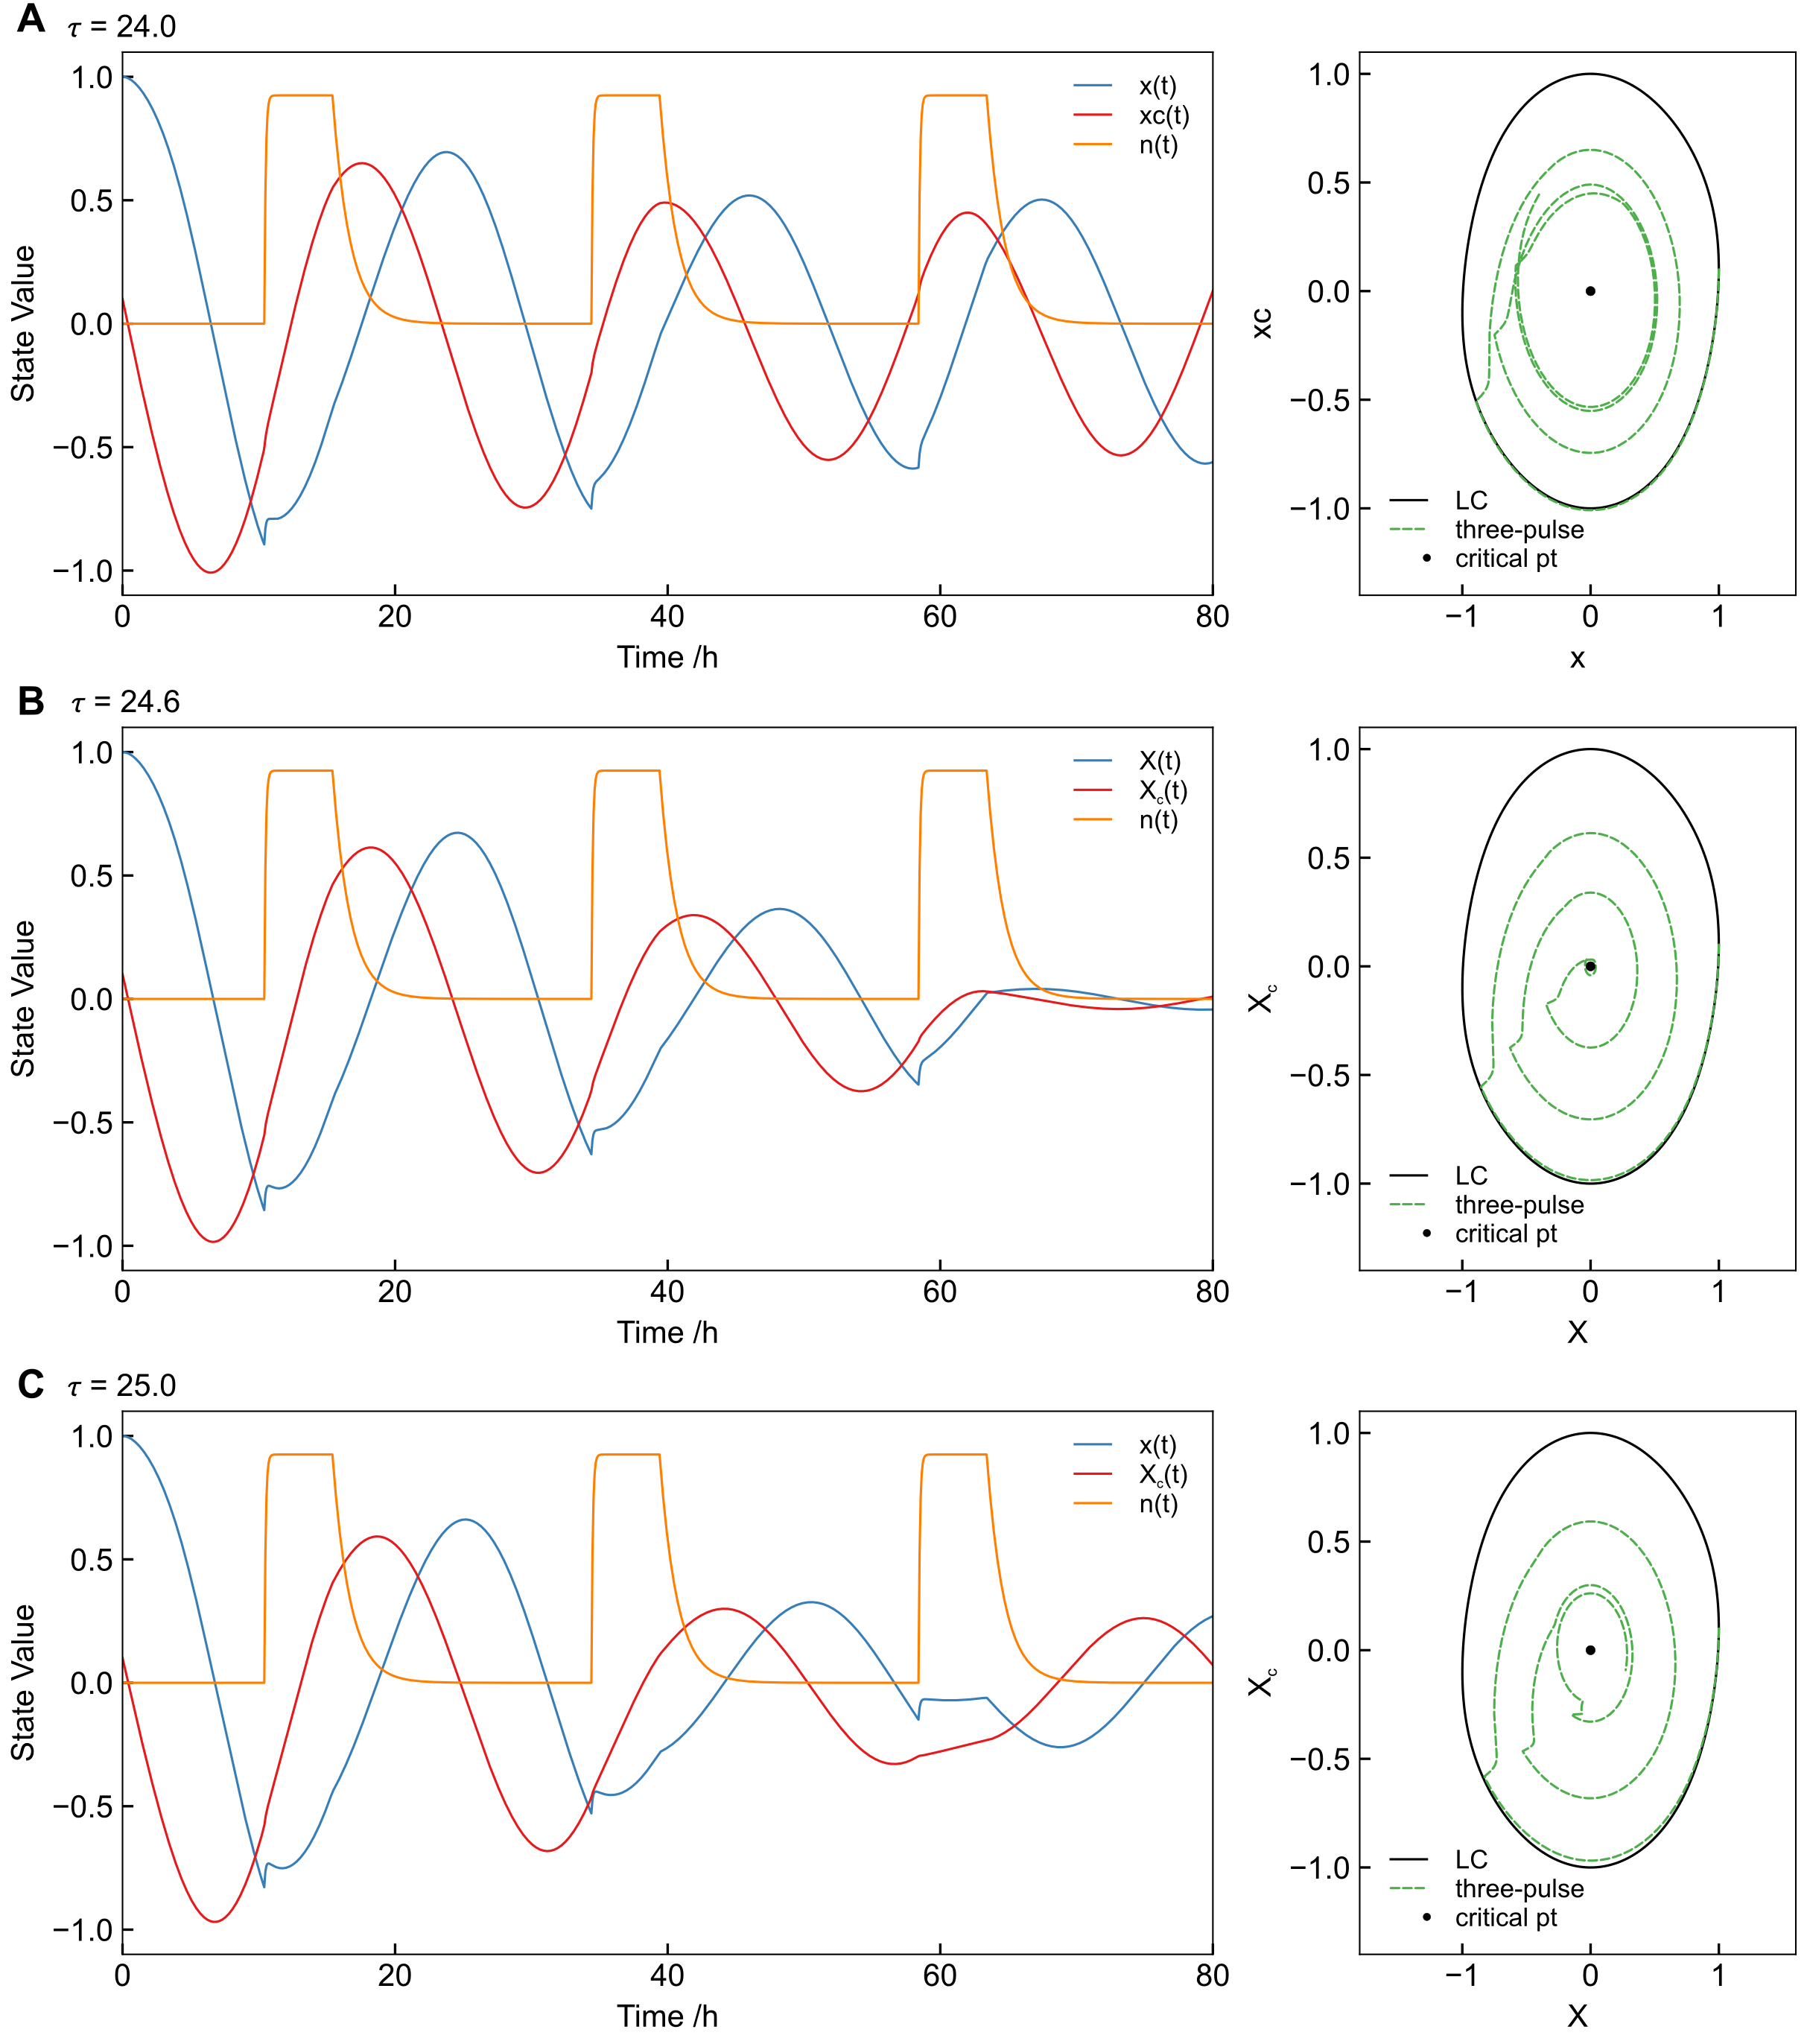
\includegraphics[width=6.5in]{chap10/figures/blind.png}
    \end{center}
        \caption{\label{fig:blind} Simulation of the three pulse experiment from \cite{Kronauer1999} demonstrates effect of period on critical resetting.
    Periods that are short (\textbf{A}) or long (\textbf{C}) do not reach the critical point, whereas an intermediate value (\textbf{B}) yields a trajectory that very nearly approaches the critical point.}
\end{figure}

\begin{figure}[p]
    \begin{center}
        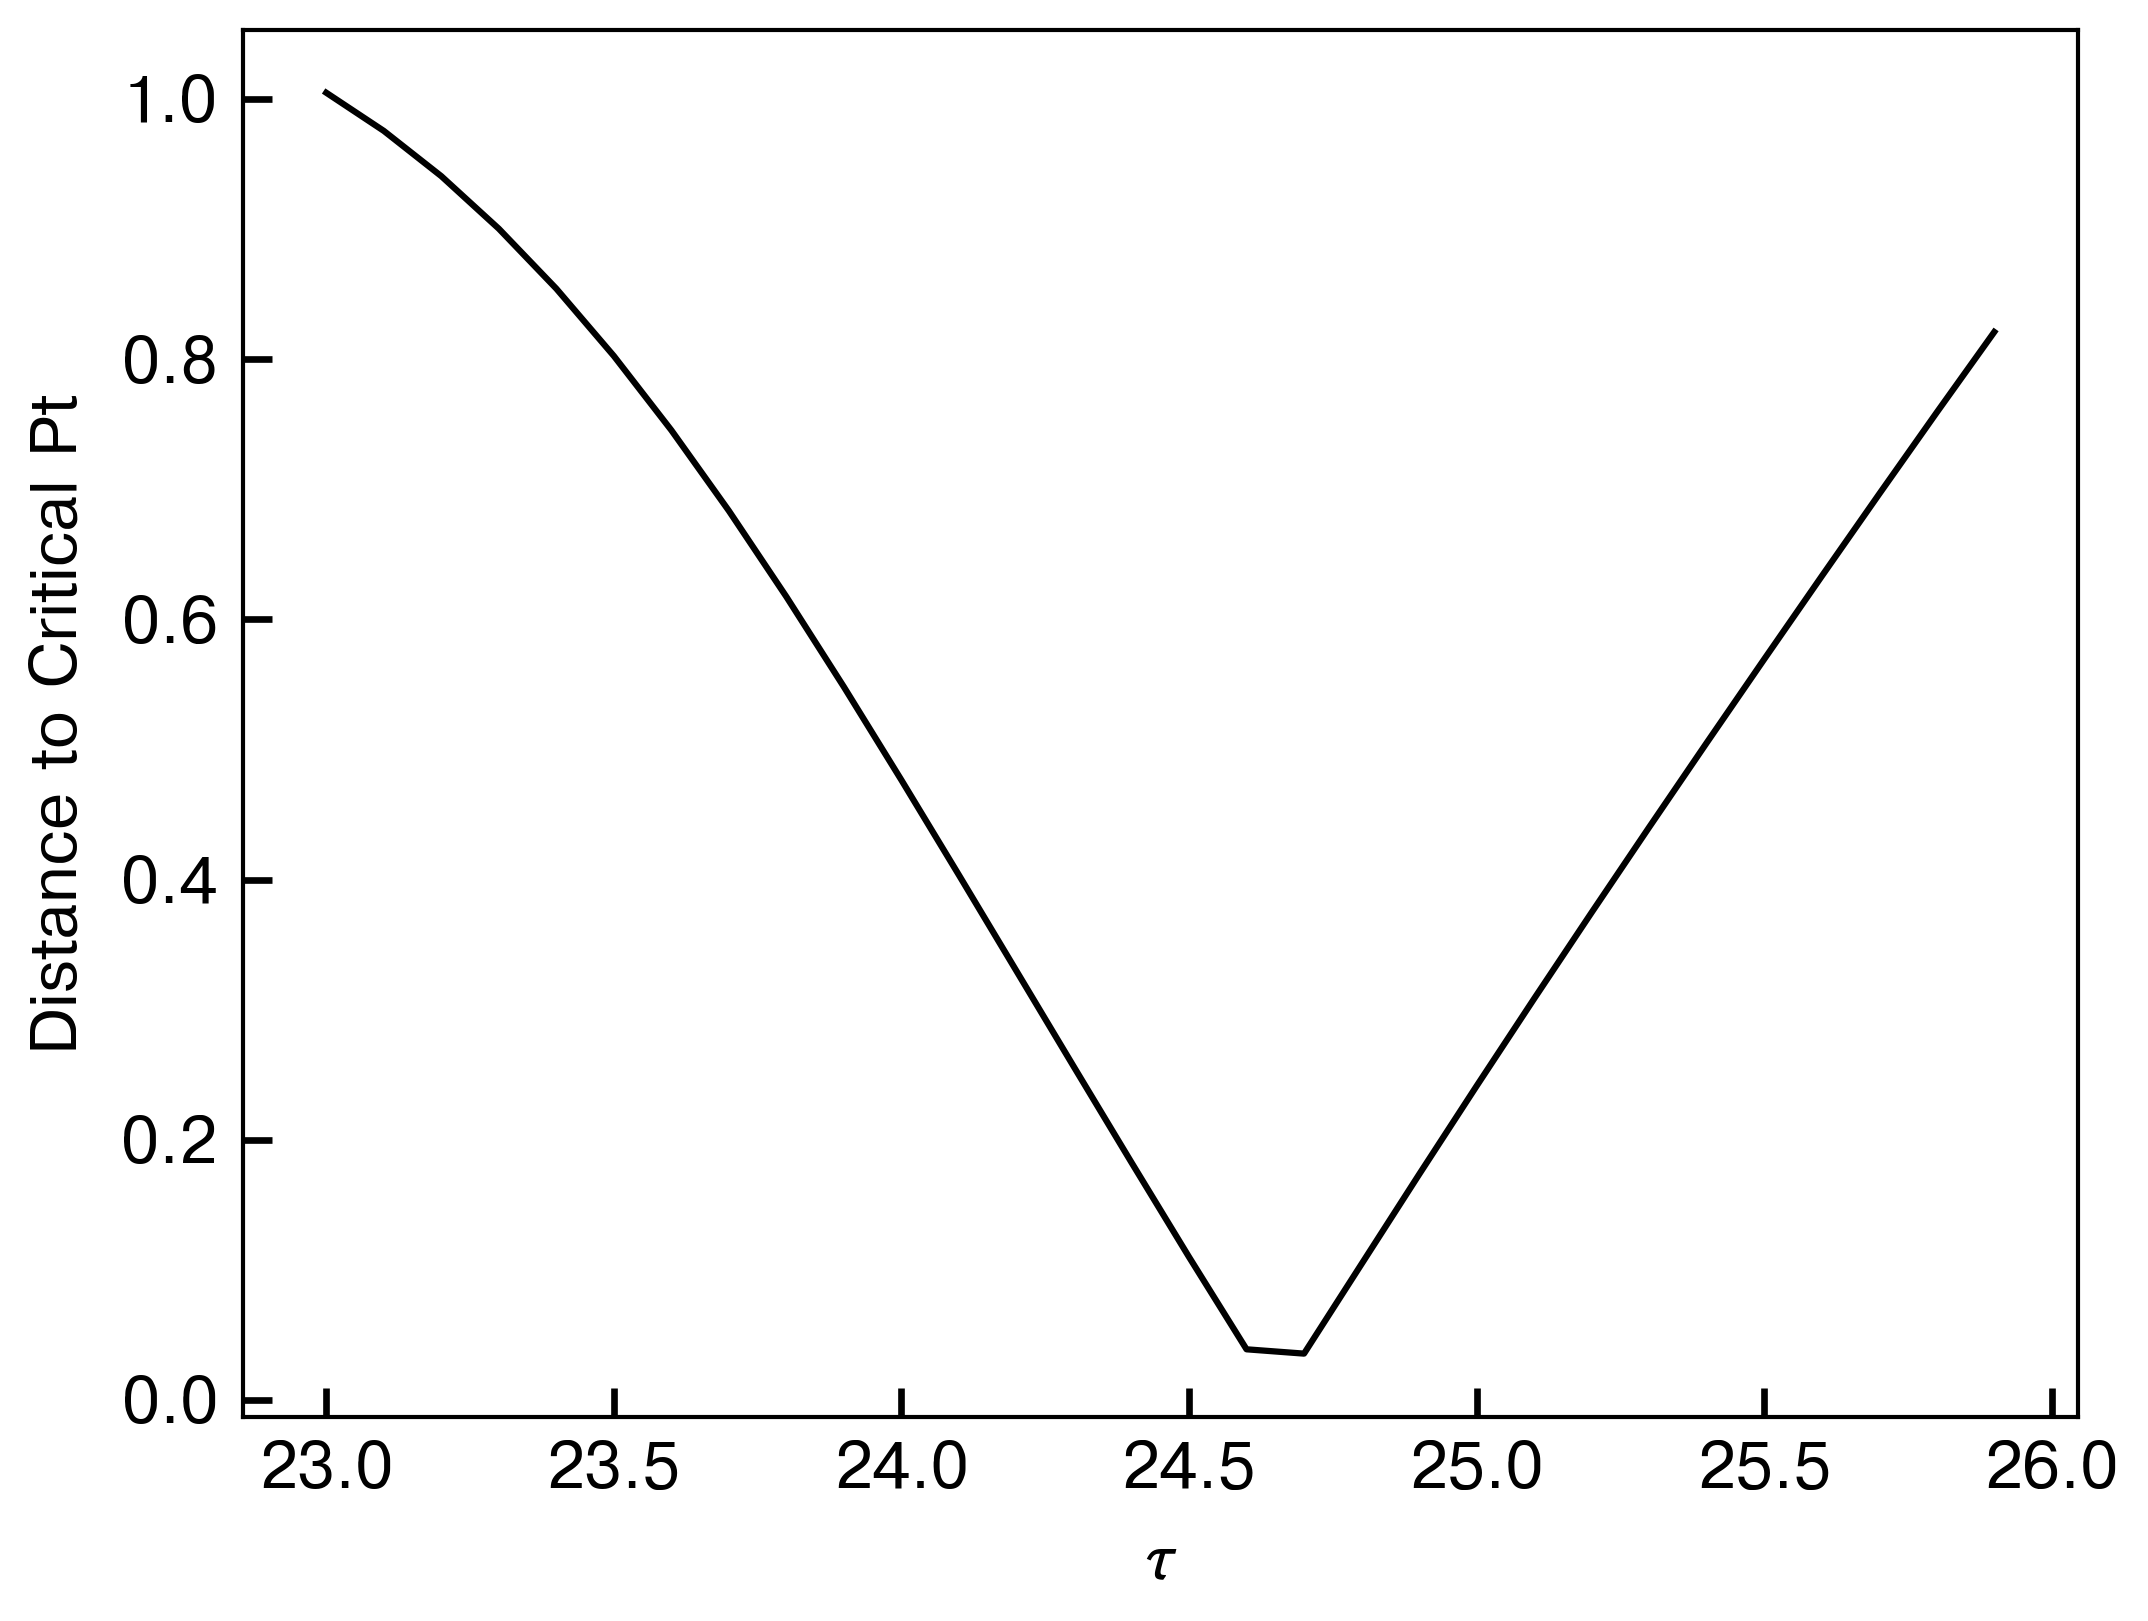
\includegraphics[width=3.5in]{chap10/figures/threepulse_sensitivity.png}
    \end{center}
        \caption{\label{fig:blind2} Simulation of the three pulse experiment from \cite{Kronauer1999} yields a plot of distance from the critical point for a range of individual periods ($\tau$).}
\end{figure}

Core body temperature minimum corresponds to the positive zero-cross of the type 1 PRC for this model (see Figure 11 in \cite{Kronauer1999}).
The critical resetting protocol (three 5-h pulses of 9500 lux 19 h apart, centered at core body temperature minimum on the first day) is therefore highly sensitive to period variability.
If the oscillatory period is too short, the 5 h pulse will occur primarily after the minimum, in the phase advance region.
This would result in the ensuing core body temperature minimum occurring even earlier due to the phase advance, and the ensuing pulse falling further into the phase advance region each time, and missing the timing that results in a critical resetting.
Likewise, if the period is too long, the pulse will be applied primarily before the minimum, incurring phase delays.
The minimum will occur later each each day, and the pulse will not be delayed, resulting in also missing the core body temperature minimum.

Three simulation examples of the three-pulse experiment are shown in Figure \ref{fig:blind}, demonstrating the effect of short period (\ref{fig:blind}A), ``just right'' period (\ref{fig:blind}B), and long period (\ref{fig:blind}C) responses to the protocol.
Human period is near 24.2 h, but varies between individuals ($24.18 \pm 0.13$ mean $\pm$ standard deviation \cite{Czeisler1999}), and so this may explain why only some individuals achieve a critical reset.

To test this further, I performed this simulation for a range of $\tau$ values and plotted the distance to the critical point following the third pulse (Figure \ref{fig:blind2}).
The results show that slight changes in the period drastically alter the timing of each pulse, and thus the final distance to the critical point.
Importantly, the ``perfect'' predicted period for achieving a critical resetting ($\approx 24.6$ h) is dependent on the whole model parameterization in addition to $\tau$, and therefore may not exactly correspond to that observed in humans.
However, I predict that the general trend will be the same: the damping of amplitudes indicative of a critical resetting will be a function of individual period, with both long and short periods unable to reach the critical point.


\subsection*{A simple feedback control scheme to achieve critical resetting}
\afterpage{
\begin{figure}[p]
    \begin{center}
        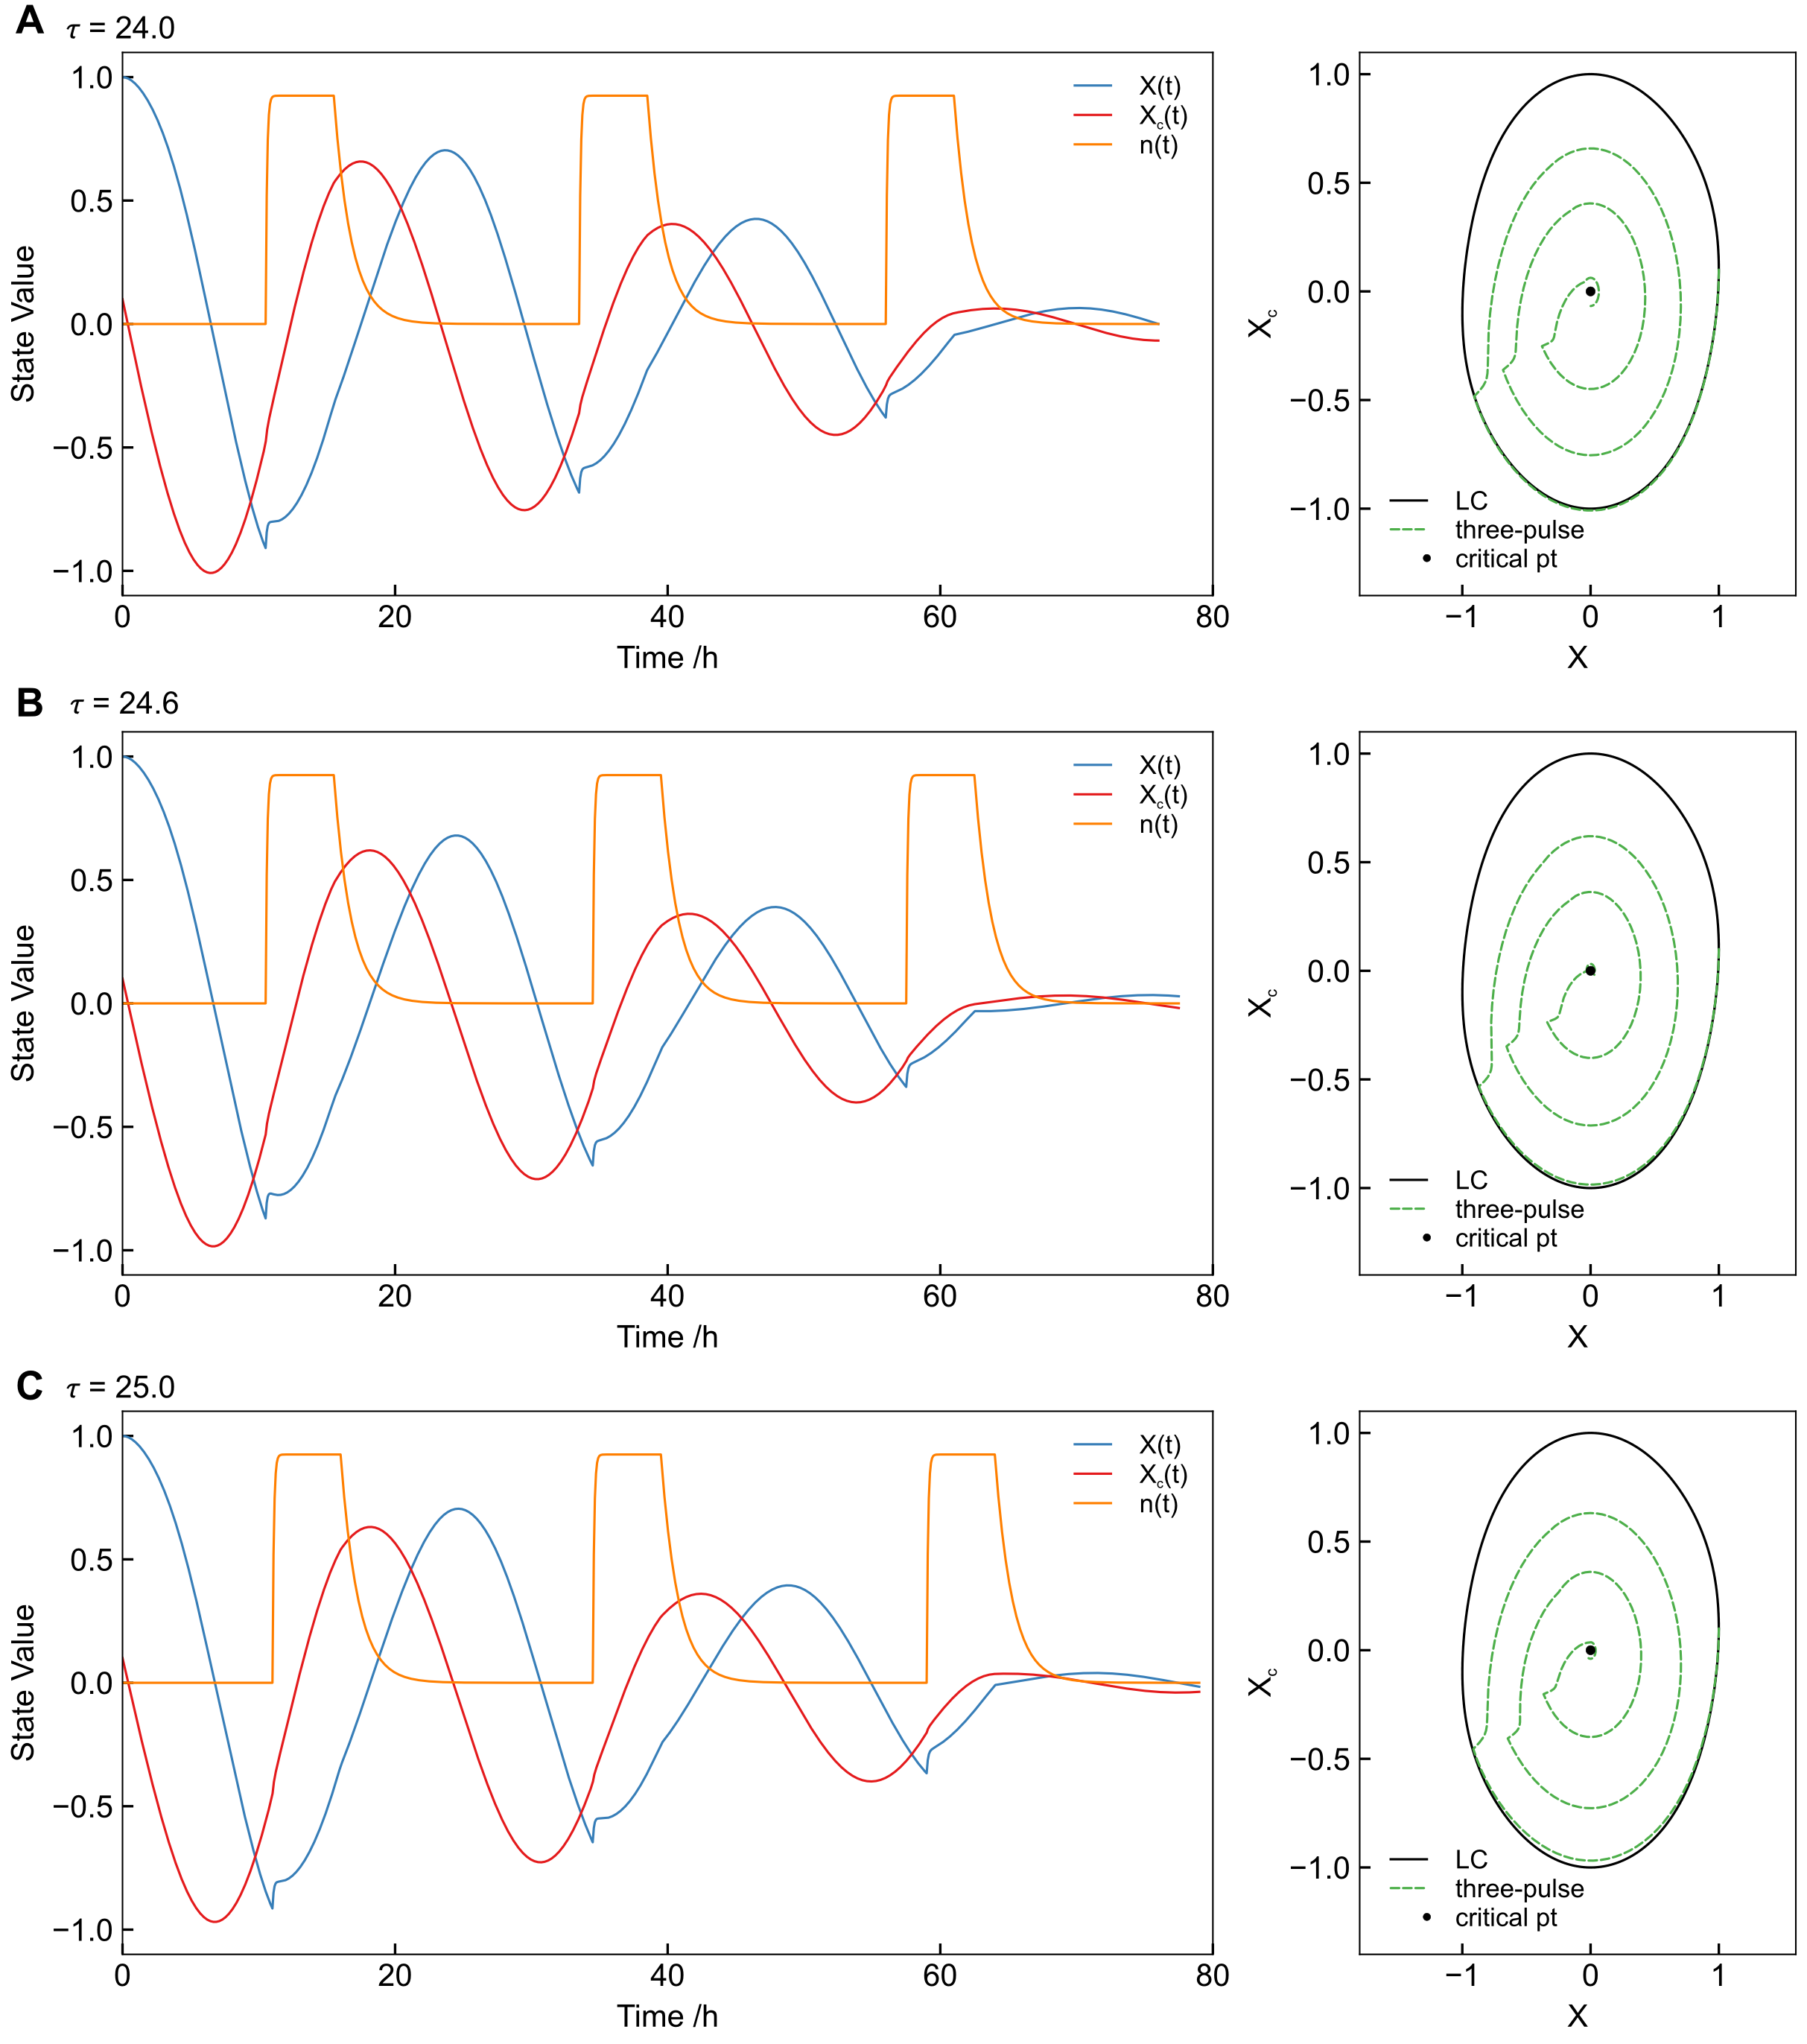
\includegraphics[width=6.5in]{chap10/figures/ctrl.png}
    \end{center}
        \caption{\label{fig:ctrl3} Simulation of the three pulse experiment from \cite{Kronauer1999} under closed-loop control.
    Oscillators with periods that are short (\textbf{A}) or long (\textbf{C}) are now able to reach the critical point comparably to that with the ``ideal'' period length of 24.6 h (\textbf{B}).}
\end{figure}
\clearpage
\begin{figure}[p]
    \begin{center}
        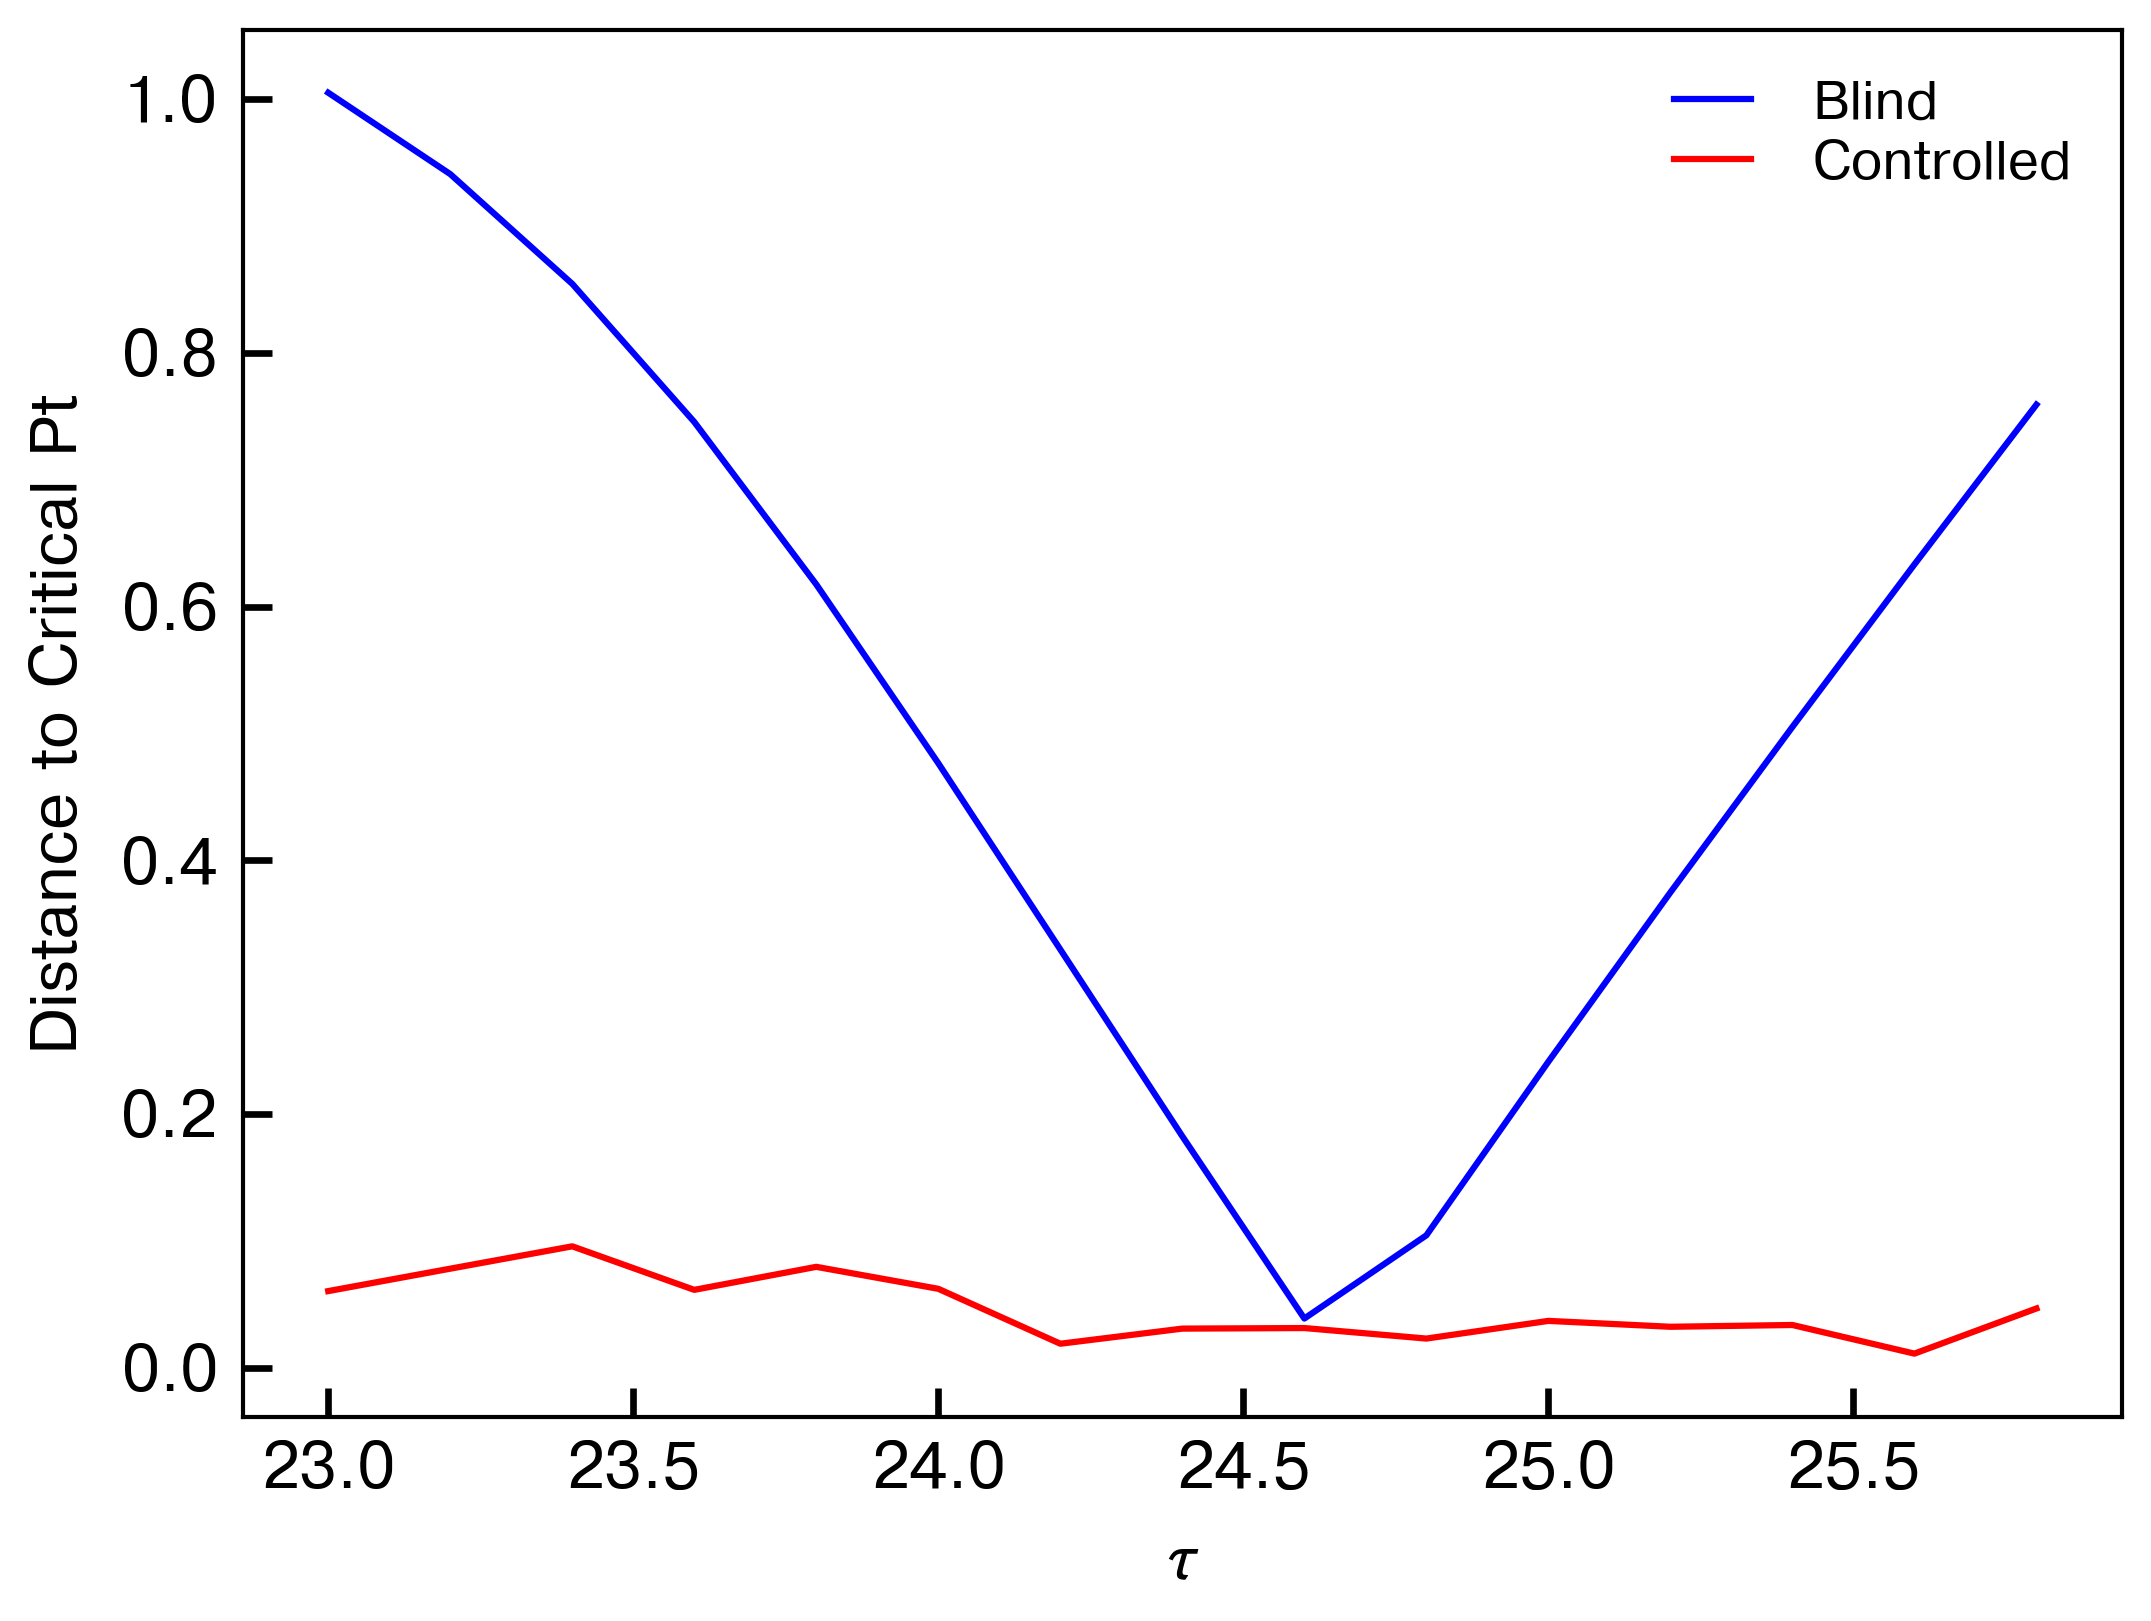
\includegraphics[width=3.5in]{chap10/figures/comparison.png}
    \end{center}
        \caption{\label{fig:ctrl32} Simulation of the three pulse experiment from \cite{Kronauer1999} either shooting blind (open-loop) or under closed-loop control yields a plot of distance from the critical point for a range of individual periods ($\tau$). Notably, the distance to the critical point is reduced in all cases.}
\end{figure}
}

Achieving a critical reset is desirable for the ability to return to the limit cycle at any phase following the resetting.
The prior result suggests that simply applying the three light pulses under feedback control would allow targeting of the core body temperature minimum, even if it were to shift following a light pulse.
This would enable critical resetting even in individuals that could not achieve it under open loop (i.e. no feedback) application of light.
Here, I tested that prediction.

To do so, I first identified the phase at which the light pulse begins for the optimal individual period ($\tau = 24.6$ h).
This phase was found to be approximately 2.66 radians, and denoted $\phi_{\text{start}}$.
I then performed feedback control simulations where the phase was calculated every 30 minutes.
When the measured phase first exceeded $\phi_{\text{start}}$, the 5 h pulse was applied.
Phase tracking resumed following the pulse. 

Figures \ref{fig:ctrl3} and \ref{fig:ctrl32} demonstrate the results of the three pulse experiment now under feedback control.
Because the application of light is now performed in closed-loop, a critical resetting is achieved irrespective of long or short oscillatory periods (Figure \ref{fig:ctrl3}A,C).
Furthermore, any oscillator with a period within physiological range is predicted to approach the critical point under closed-loop control (Figure \ref{fig:ctrl32}).


These very encouraging results warrant further examination, and work is currently underway to (i) design a feedback control protocol based on amplitude response curves rather than phase comparison, and (ii) determine if it is feasible to implement such a strategy in a clinical or ambulatory setting.
Toward aim (i), the infinitesimal parametric amplitude response curve can be calculated for this model for the light input (term $B(t)$).
This might allow us to better guide the delivery of light based on properties of the oscillator, rather than simply relying on repeating a clinical protocol. 
In approaching aim (ii), the essential element for implementing this protocol is the ability to sense phase sufficiently accurately for achieving a critical reset.
A first step, then, would be examining exactly how sensitive critical resetting is to mistimed application of the light pulse due to imprecisions in on-line phase sensing.
The controller, as currently formulated, applies feedback within a half hour of the desired phase.
This is sufficient to achieve critical resetting, as errors do not compound from cycle-to-cycle, unlike the open loop case.

\section{Conclusion}
In sum, closed-loop circadian control is a relatively unexplored problem at the interface of control theory and systems biology. 
Whether by incurring incremental shifts via a pharmaceutical stimulus, or by exploiting the oscillatory critical point, circadian control has the potential to improve quality of life for shift workers or any individual attempting to maximize cognitive or physical performance. 
Though significant challenges remain in implementing closed-loop circadian control, the technology to do so exists.
It is my hope that the research contained in this dissertation is an incremental step in the direction of understanding and control over the circadian rhythms that affect nearly every living organism.













